\documentclass[a4paper]{article}

\usepackage[english]{babel}
\usepackage[utf8]{inputenc}
\usepackage{amsmath}
\usepackage{graphicx}

\title{
	Project 02 \\
	\bigskip
	\normalsize APSC 607 Fall 2017
}

\author{Seth Goodman}

\date{\today}

\begin{document}
\maketitle


%\begin{abstract}
%\end{abstract}

\section{Introduction}
\label{sec:introduction}

Some text\cite{burden2010}.

\begin{equation}
f(x) = e^{2x} * sin(3x)
\label{eq:eqb}
\end{equation}

\begin{equation}
f(x) = \frac{1}{x+4}
\label{eq:eqa}
\end{equation}


\begin{figure}
\centering
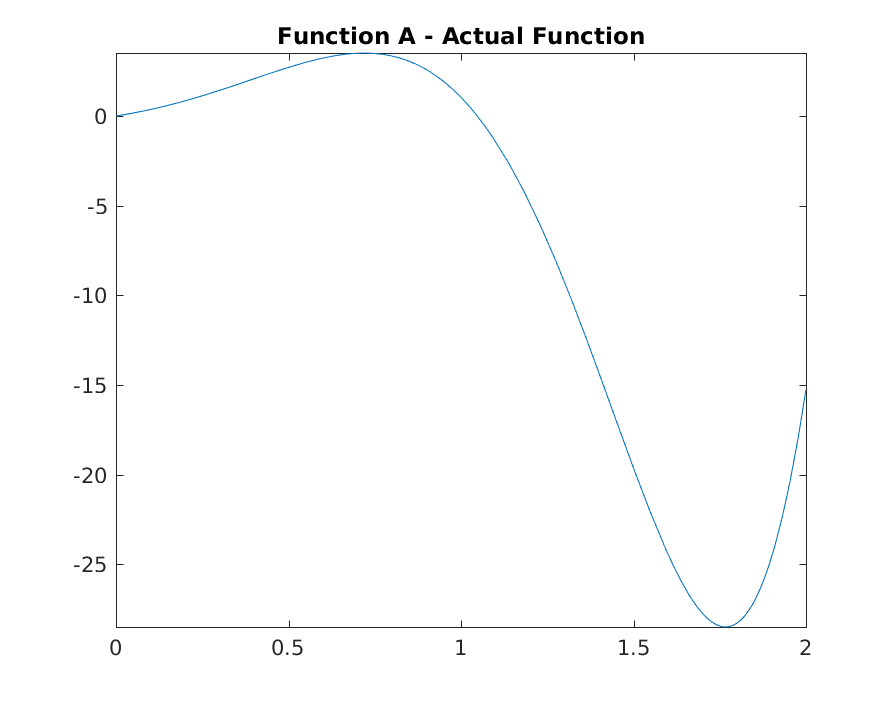
\includegraphics[width=1\textwidth]{../output/a_actual.png}
\caption{\label{fig:data}caption text}
\end{figure}




\section{Methods}
\label{sec:methods}

\subsection{Trapezoidal}
Here, explain the concept of a 2-DEG in GaAs/AlGaAs. What is a 2-DEG and why does it arise?

\subsection{Midpoint}
Explain the classical Hall effect in your own words. What do I measure at $B=0$? And what happens if $B>0$? Which effect gives rise to the voltage drop in the vertical direction?

\subsection{Simpson's}
Explain the IQHE in your own words. What does the density of states look like in a 2-DEG when $B=0$? What are Landau levels and how do they arise? What are edge states? What does the electron transport look like when you change the magnetic field? What do you expect to measure?

\subsection{Adaptive Simpson's}
Explain the IQHE in your own words. What does the density of states look like in a 2-DEG when $B=0$? What are Landau levels and how do they arise? What are edge states? What does the electron transport look like when you change the magnetic field? What do you expect to measure?


\newpage
\section{Results}
\label{sec:results}
\subsection{How to Include Figures}

First you have to upload the image file (JPEG, PNG or PDF) from your computer to writeLaTeX using the upload link the project menu. Then use the includegraphics command to include it in your document. Use the figure environment and the caption command to add a number and a caption to your figure. See the code for Figure \ref{fig:frog} in this section for an example.

\begin{figure}
\centering
\includegraphics[width=0.3\textwidth]{frog.jpg}
\caption{\label{fig:frog}This frog was uploaded to writeLaTeX via the project menu.}
\end{figure}

\subsection{How to Make Tables}

Use the table and tabular commands for basic tables --- see Table~\ref{tab:widgets}, for example.

\begin{table}
\centering
\begin{tabular}{l|r}
Item & Quantity \\\hline
Widgets & 42 \\
Gadgets & 13
\end{tabular}
\caption{\label{tab:widgets}An example table.}
\end{table}

\subsection{How to Write Mathematics}

\LaTeX{} is great at typesetting mathematics. Let $X_1, X_2, \ldots, X_n$ be a sequence of independent and identically distributed random variables with $\text{E}[X_i] = \mu$ and $\text{Var}[X_i] = \sigma^2 < \infty$, and let

\begin{equation}
S_n = \frac{X_1 + X_2 + \cdots + X_n}{n}
      = \frac{1}{n}\sum_{i}^{n} X_i
\label{eq:sn}
\end{equation}

denote their mean. Then as $n$ approaches infinity, the random variables $\sqrt{n}(S_n - \mu)$ converge in distribution to a normal $\mathcal{N}(0, \sigma^2)$.

The equation \ref{eq:sn} is very nice.

\subsection{How to Make Sections and Subsections}

Use section and subsection commands to organize your document. \LaTeX{} handles all the formatting and numbering automatically. Use ref and label commands for cross-references.

\subsection{How to Make Lists}

You can make lists with automatic numbering \dots

\begin{enumerate}
\item Like this,
\item and like this.
\end{enumerate}
\dots or bullet points \dots
\begin{itemize}
\item Like this,
\item and like this.
\end{itemize}
\dots or with words and descriptions \dots
\begin{description}
\item[Word] Definition
\item[Concept] Explanation
\item[Idea] Text
\end{description}

We hope you find write\LaTeX\ useful, and please let us know if you have any feedback using the help menu above.


\begin{thebibliography}{9}
\bibitem{burden2010}
  Burden, R., Faires, J., Numerical Analysis 9th Edition. 2010

\end{thebibliography}
\end{document}
